% !TEX TS-program = XeLaTeX
% !TEX spellcheck = en-US
\documentclass[aspectratio=169]{beamer}

\usetheme{bi}

\title{Lecture 8:\\ Random forests and Extra trees}
\institute{GRA4160: Predictive modelling with machine learning}
\date{February 29th 2023}
\author{Vegard H\o ghaug Larsen}

\begin{document}

\maketitle

\frame{
	\frametitle{Plan for today:}

	\begin{itemize}
		\item Recap decision trees
		\item Random forests
		\item Extra trees
	\end{itemize}
}

\frame{
	\frametitle{Recap: Decision trees}
	\begin{itemize}
		\item The tree is built by recursively splitting the data into smaller subsets based on the feature that provides the most information gain
		\pause
		\item The splitting is done by choosing a threshold value for each feature, and splitting the data into two subsets based on whether the feature value is above or below the threshold value
		\pause
		\item The leaf nodes of the tree contain the final decision or prediction for each class label or numerical value
		\pause
		\item Decision trees are easy to interpret and visualize, but can suffer from overfitting and bias if not pruned or regularized properly
	\end{itemize}
}

\frame{
	\frametitle{Visualization of decision trees}

	\href{https://github.com/parrt/dtreeviz}{https://github.com/parrt/dtreeviz}

    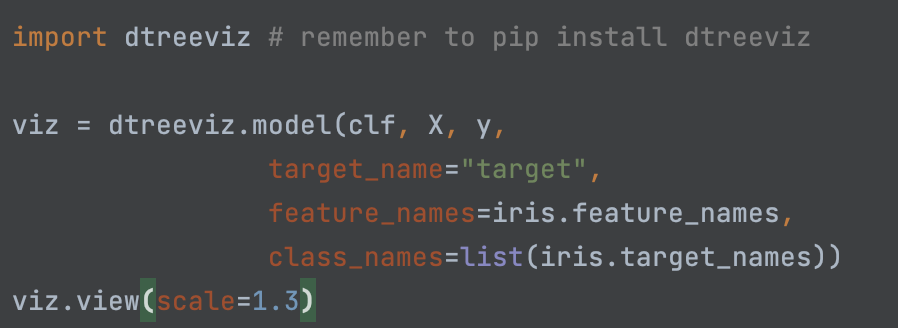
\includegraphics[width=0.8\textwidth]{figures/code_dttreeviz.png}
}

\frame{
	\frametitle{Visualization of decision trees}

    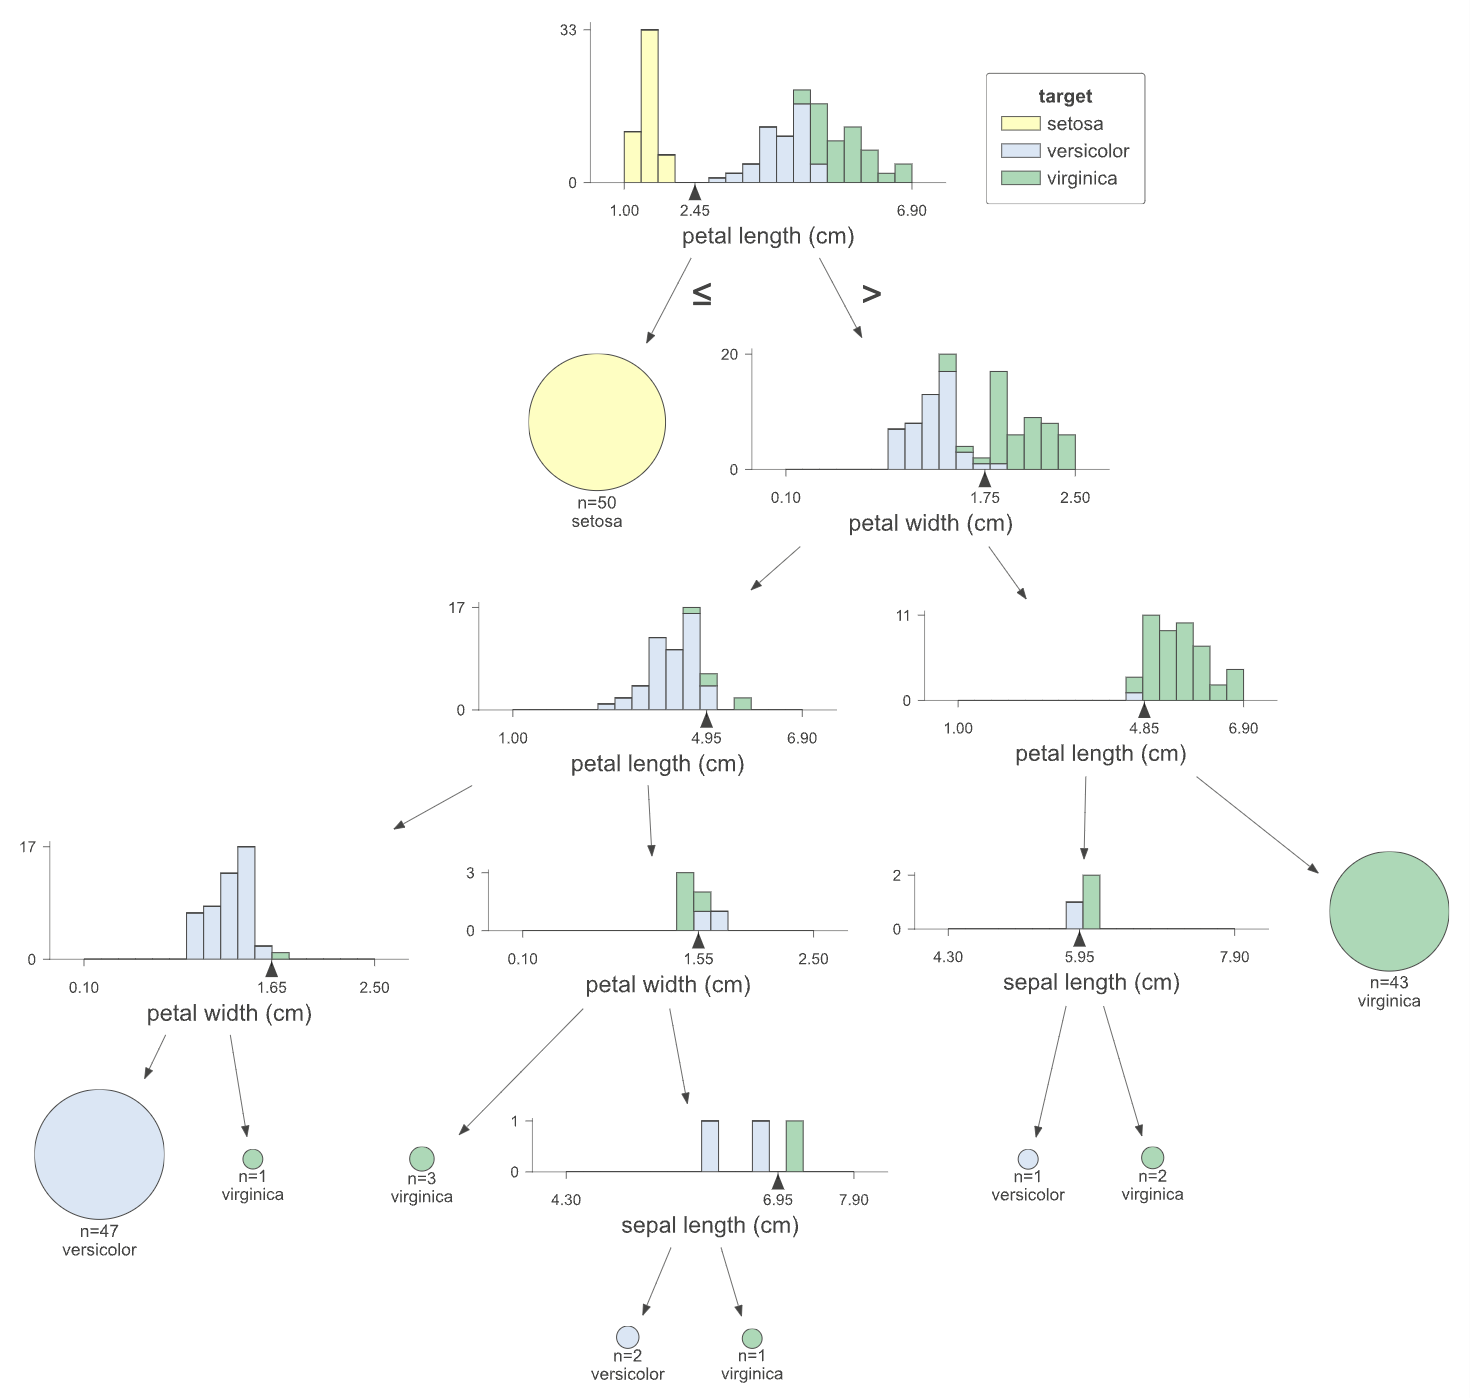
\includegraphics[width=0.5\textwidth]{figures/decision_tree.png}
}

%\frame{
%	\frametitle{Algorithms: CART and ID3}
%	\begin{itemize}
%		\item CART stands for Classification and Regression Trees
%		\item ID3 stands for Iterative Dichotomiser 3
%		\item Both algorithms are used to build decision trees
%		\item ID3 is a greedy algorithm that builds the tree by choosing the feature that provides the most information gain at each node
%		\item CART is a greedy algorithm that builds the tree by choosing the feature that provides the most information gain at each node, but it can also handle numerical features
%		\item CART can be used to build both classification and regression trees
%	\end{itemize}
%}

\frame{
	\frametitle{Decision trees $\rightarrow$ Random forests}
	\begin{itemize}
		\item To create a Random Forest, we need to generate multiple decision trees
		\pause
		\item Using standard  Bagging to generate multiple decision trees, will give us trees that are highly correlated with each other
		\pause
		\item In Bagging we create subsets of the training data by randomly selecting samples with replacement (known as bootstrapping)
		\pause
		\item Each subset will have the same number of samples as the original training data, but some samples may be repeated
		\pause
		\item Random Forest is a modified form of bagging that creates ensembles of \textbf{independent decision trees}
	\end{itemize}
}

\frame{
	\frametitle{De-correlated trees}
	\begin{enumerate}
		\item Each tree in the forest is built from a bootstrapped subset of the training data (same as Bagging)
		\pause
		\item For each tree, at each split, we randomly select a set of predictors from the full set of predictors
		\pause
		\item From these predictors, we select the optimal predictor and the optimal corresponding threshold for the split
		\pause
		\item The number of predictors to consider at each split is typically the square root of the total number of predictors
	\end{enumerate}
}


\frame{
	\frametitle{Random forests}
	\begin{itemize}
		\item For each of the bootstrapped training datasets, we build a decision tree were we randomly select a subset of features to consider, rather than considering all features
		\pause
		\item The final prediction of the Random Forest model is obtained by aggregating the predictions of all the decision trees in the forest
		\pause
		\item Each decision tree in the forest votes on the class label of the input data point, and the class with the most votes is the predicted class
	\end{itemize}
}

\frame{
	\frametitle{Hyper-parameters for  random forests}
	\begin{itemize}
		\item The number of trees in the forest (\texttt{n\_estimators}). A larger value, leads to more trees in the forest, which can lead to overfitting
		\pause
		\item The number of features to consider at each split (\texttt{max\_features}). A smaller value, leads the decision trees to have fewer but more general nodes
		\pause
		\item The maximum depth of each tree (\texttt{max\_depth}). A larger value, leads the decision trees to have deeper nodes, which can lead to overfitting
		\pause
		\item The minimum number of samples required to split a node (\texttt{min\_samples\_split}). A larger value, leads the decision trees to have fewer but more general nodes
		\pause
		\item The minimum number of samples required at each leaf node (\texttt{min\_samples\_leaf}). A larger value, leads the decision trees to have fewer but more general nodes
	\end{itemize}
}

\frame{
	\frametitle{Extra trees}
	\begin{itemize}
		\item Stands for Extremely Randomized Trees
		\pause
		\item Builds a collection of decision trees using a random subset of features at each node of the tree (like with Random Forest)
		\pause
		\item The main difference between Random Forest and Extra Trees lies in the way they generate random splits at each node of the decision trees
		\pause
		\item The splits at each node are chosen randomly, rather than using the optimal split as in Random Forest
		\pause
		\item Selects a threshold value for each feature at each node and chooses the one that maximizes the information gain
		\pause
		\item Leads to a more randomized and less biased decision tree, which can be more effective at reducing overfitting
	\end{itemize}
}

\end{document}